\documentclass{standalone}
\usepackage{tikz}

\usetikzlibrary{calc}

\begin{document}

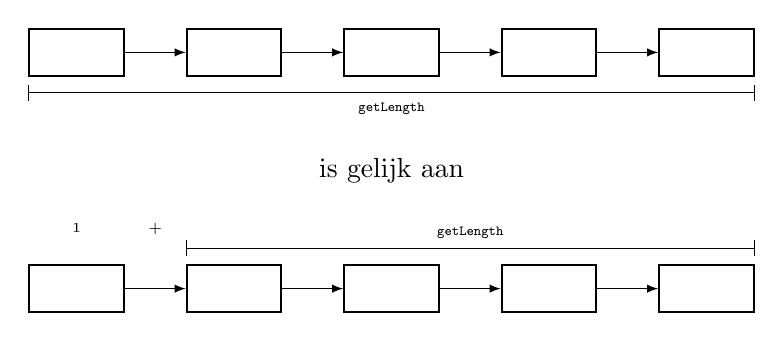
\begin{tikzpicture}[wagon/.style={minimum width=1.2cm,minimum height=0.6cm,draw,black,thick},
                    link/.style={-latex,thin},
                    address/.style={font=\tiny,circle,thin,fill=white}]

  \foreach[count=\i] \c in {20,30,25,55,5} {
    \pgfmathparse{(\i-1)*2}\let\x\pgfmathresult
    \node[wagon] (w\i) at (\x,0) {};
  }
  \foreach \i in {1,2,3,4} {
    \pgfmathparse{int(\i+1)}\let\j\pgfmathresult
    \draw[link] (w\i.east) -- (w\j.west);
  }

  \draw[|-|] ($ (w1.south west) + (0,-.2) $) -- ($ (w5.south east) + (0,-.2) $)
             node[midway,below] {\tt\tiny getLength};

  \begin{scope}[yshift=-3cm]
    \foreach[count=\i] \c in {20,30,25,55,5} {
      \pgfmathparse{(\i-1)*2}\let\x\pgfmathresult
      \node[wagon] (ww\i) at (\x,0) {};
    }
    \foreach \i in {1,2,3,4} {
      \pgfmathparse{int(\i+1)}\let\j\pgfmathresult
      \draw[link] (ww\i.east) -- (ww\j.west);
    }
  \end{scope}

  \draw[|-|] ($ (ww2.north west) + (0,.2) $) -- ($ (ww5.north east) + (0,.2) $)
             node[midway,above] (getLength) {\tt\tiny getLength};
  \path let \p1 = (getLength), \p2 = (ww1.north), \p3 = ($ (ww1.north) ! .5 ! (ww2.north) $) in
        node[anchor=south,anchor=base] at (\x2,\y1) {\tiny 1}
        node[anchor=south,anchor=base] at (\x3,\y1) {\tiny +};

  \node at ($ (ww1.north west) ! .5 ! (w5.south east) $) {is gelijk aan};        
\end{tikzpicture}

\end{document}